\documentclass[10pt,a4paper]{article}

\usepackage[spanish]{babel}
\usepackage[utf8]{inputenc}
\usepackage{geometry}
\usepackage{url}
\usepackage{amsmath}
\usepackage{graphicx}
\usepackage{listings}
\usepackage{color}
\usepackage{multicol}
\definecolor{grey}{rgb}{0.8,0.8,0.8}
\usepackage{listings}
\usepackage{pdfpages}
\usepackage{csquotes}
\usepackage{float}


% Configuración de lstlisting:

\lstset{
language=C,
tabsize=4,
numbers=left,
stepnumber=5,
keywordstyle=\color{blue},
frame=single,
basicstyle=\fontsize{11}{13}\ttfamily\footnotesize,
showspaces=false,
showstringspaces=false,
captionpos=b,
breaklines=true
}

\title{\textbf{Trabajo Práctico 0: Infraestructura básica}}

\author{Santiago Aguilera, \textit{Padrón Nro. 95795}\\
        \texttt{marquito.santi@gmail.com}\\
        Agustina Barbetta, \textit{Padrón Nro. 96528}\\
        \texttt{agustina.barbetta@gmail.com}\\
        Manuel Porto, \textit{Padrón Nro. 96587}\\
        \texttt{manu.porto94@hotmail.com}\\
        \\[2.5ex]
        \normalsize{2do. Cuatrimestre de 2016}\\
        \normalsize{66.20 Organización de Computadoras}\\
        \normalsize{Facultad de Ingeniería, Universidad de Buenos Aires}\\
       }


\begin{document}
\date{13 de Septiembre del 2016}

\maketitle

\thispagestyle{empty}
\begin{abstract}
El presente trabajo práctico consiste en crear una aplicación, en ISO C, totalmente personalizable capaz de dibujar los conjuntos fractales de Julia sobre una imagen de formato PGM.

El código del trabajo se encuentra en el siguiente repositorio: \\
\texttt{https://github.com/saantiaguilera/fiuba-orga-pc-julia-set}.\\
\end{abstract}

\pagebreak

\tableofcontents

\pagebreak

\section{Introducción}
El principal objetivo de este trabajo es familiarizarse con las herramientas de software que usaremos en los siguientes prácticos\cite{Gxemul}\cite{NetBSD}, implementando un programa y su correspondiente documentación que resuelvan el problema descripto más adelante.

\section{Conjunto de Julia}
El programa a implementar debe generar distintas imágenes pertenecientes a los conocidos `conjuntos de Julia`.
\begin{displayquote}
Los conjuntos de Julia, así llamados por el matemático Gaston Julia, son una familia de conjuntos fractales que se obtienen al estudiar el comportamiento de los números complejos al ser iterados por una función holomorfa.

El conjunto de Julia de una función holomorfa $f$, está constituido por aquellos puntos que bajo la iteración de $f$, tienen un comportamiento 'caótico'. El conjunto se denota $J(f)$.

En el otro extremo se encuentra el conjunto de Fatou (en honor del matemático Pierre Fatou), que consiste de los puntos que tienen un comportamiento 'estable' al ser iterados. El conjunto de Fatou de una función holomorfa $f$, se denota $F(f)$ y es el complemento de $J(f)$.\cite{Juli}
\end{displayquote}

\section{Programa}
El programa a escribir, en lenguaje C, recibirá al momento de ejecutarse distintos argumentos para modificar el archivo generado o las condiciones del conjunto de Julia.

Los mismos son:

\begin{itemize}
    \item -o: Obligatorio. Archivo de salida para la imagen. Debe terminar con .pgm. Si el argumento es '-' se utilizara la salida estándar (stdout).
    
    \item -r: Opcional. Resolución de la imagen de salida. Por defecto sera 640x480 px.
    
    \item -c: Opcional. Centro del set de la partición del plano complejo. Por default sera 0+0i.
    
    \item -C: Opcional. Parámetro C de la ecuación de iteración (correspondiente a la familia cuadrática). Por defecto se usara 0.285+0.01i
    
    \item -w: Opcional. Ancho del rectángulo del set en el plano real. Por defecto sera 4.
    
    \item -H: Opcional. Alto del rectángulo del set en el plano complejo. Por defecto sera 4.
    
    \item -h: Opcional. Help. Brinda información detallada del uso de cada parámetro y ejemplos.
    
    \item -v: Opcional. Versión del programa.
\end{itemize}

\subsection{Modo de uso}
Si no se tiene el ejecutable, para generarlo se debe correr (dentro de donde están los archivos fuente, en caso de clonar el repositorio del trabajo, \texttt{cd src/}) \texttt{make}.

Una vez que se tenga el archivo ejecutable. Una ejecución básica, usando los parámetros por defecto será:

\texttt{./tp0 -o filename.pgm}

Si se desea personalizar los parámetros del conjunto de Julia o de la imagen, se pueden obtener mediante:

\texttt{./tp0 -h}

Allí se encuentra toda la documentación detallada para personalizar el programa.

\subsection{Diseño}
A continuación se describe cada uno de los módulos implementados para la realización del programa.

\subsubsection{Complex}
En el modulo complex.c se implemento la estructura del numero complejo junto con algunas de sus operaciones básicas ya que la misma no esta soportada de manera nativa en el lenguaje C.

\subsubsection{Decoder}
En el modulo decoder.c se define la lógica para decodificar una imagen en base a los parámetros recibidos y escribirla sobre un archivo de salida. El mismo creará una imagen de formato PGM (Formato "P2") de dimensiones 640x480 píxeles (el tamaño puede modificarse pasando por parámetro \texttt{-r widthxheight}). A su vez, se encontrará centrada en el 0+0i y el recinto sobre el que se iterará para obtener el conjunto de Julia es de 4 tanto de largo como de ancho (Para usar valores distintos para el centro o las dimensiones, se puede ejecutar agregando \texttt{-c x+yi -w width -H height})

El conjunto de Julia se calcula iterando sobre una familia de polinomios cuadrados dados de la forma

$$z_{n+1} = z_{n}^{2} + c$$

$$c = 0.285 + 0.01i$$

Si se desea cambiar el valor de c. Por parámetro se deberá ingresar \texttt{-C x+yi}. La condición de corte utilizada por el decodificador será, que el brillo no sea mayor a 255 (Valor máximo utilizado por la imagen PGM para el brillo) y que $abs(z) <= 2$. 

\subsubsection{Main}
En el módulo main.c se define la función que da inicio al programa, inmediatamente después, por medio de \texttt{getopt\_long} se cicla entre todos los \textit{flags} recibidos por parámetro, definiendo el flujo correspondiente del programa. El beneficio de esta función es que permite al usuario escribir las opciones en cualquier orden. Cabe aclarar que, si se utilizan los \textit{flags} de ayuda o versión, el programa devolverá estos datos sin importar que se hayan ingresado los parámetros para una codificación o decodificación.\\
Además, el módulo contiene funciones para mostrar el mensaje de ayuda (\texttt{show\_help()}), la versión del programa (\texttt{show\_version()}) y la función \texttt{write\_image(...)} encargada de escribir los resultados.

\subsection{Compilación}
Se provee de un \textit{Makefile} para la compilación del proyecto, el mismo cuenta con un\textit{ phony target} para limpiar los archivos generados (\texttt{make clean}) y el target \textit{phony all} que (por más que sea \textit{phony}) generará un ejecutable '\texttt{tp0}' y los archivos del linker necesarios (\texttt{make} o \texttt{make all}).

En caso de compilar el proyecto en BSD, se deben realizar los mismos pasos pero reemplazando el comando \texttt{make} por \texttt{gmake} ya que el \texttt{make} de BSD no es el mismo al que se encuentra en los sistemas Linux, que es GNU make. Entonces, para utilizar este ultimo en BSD se debe llamar a \texttt{gmake}. 

\subsection{Pruebas}
Se creó una \textit{test-suite} en bash para testear casos borde de los parámetros y que el programa funcione correctamente. 

Para correrla simplemente hay que compilar el proyecto previamente, darle permisos al \textit{script} (de ser necesarios, \texttt{chmod u+x run\_tests.sh}) y correrlo de forma normal (\texttt{bash run\_tests.sh}). El mismo irá dando información sobre cada test corrido y su estado.

Se borró, de la \textit{test suite} previa, un test que validaba que no se pudiese escribir un archivo protegido (y se retornara información al respecto de la falla), debido a que en BSD el root no es afectado por \texttt{chmod}. Estuvimos buscando si podíamos evitar que el usuario lo pueda editar, y es posible pero los comandos son exclusivos de cada OS asi que preferimos ignorar el test.

A continuación se incluye una imagen del caso default pedido por el trabajo. El mismo fue generado mediante \texttt{./tp0 -o img.pgm}.

\begin{figure}[H]
\centering
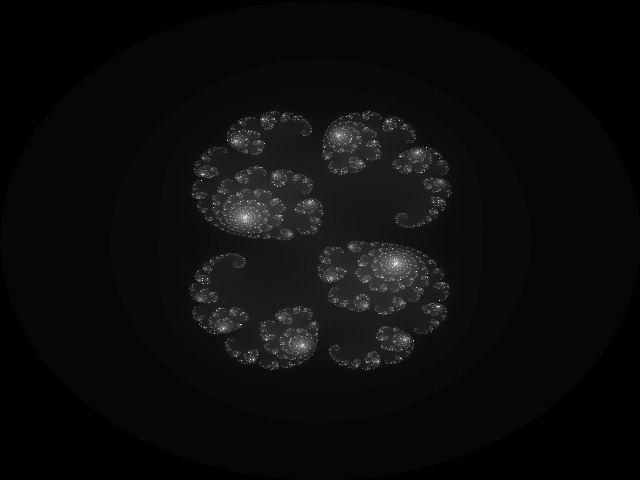
\includegraphics[width=\columnwidth]{juli.png}
\caption{Resultado por default: img.pgm}
\end{figure}

\section{Apéndices}

\subsection{Código fuente}
El código a continuación se encuentra también en el repositorio del trabajo: \\
\texttt{https://github.com/saantiaguilera/fiuba-orga-pc-julia-set}.\\

\lstinputlisting[language=C,caption=main.c]{main.c}
\lstinputlisting[language=C,caption=complex.h]{complex.h}
\lstinputlisting[language=C,caption=complex.c]{complex.c}
\lstinputlisting[language=C,caption=decoder.h]{decoder.h}
\lstinputlisting[language=C,caption=decoder.c]{decoder.c}



\subsection{Código MIPS assembly}
A continuación adjuntamos el código assembly del módulo \texttt{decoder.c}
\lstinputlisting[caption=decoder.s]{decoder.s}

\subsection{Enunciado}
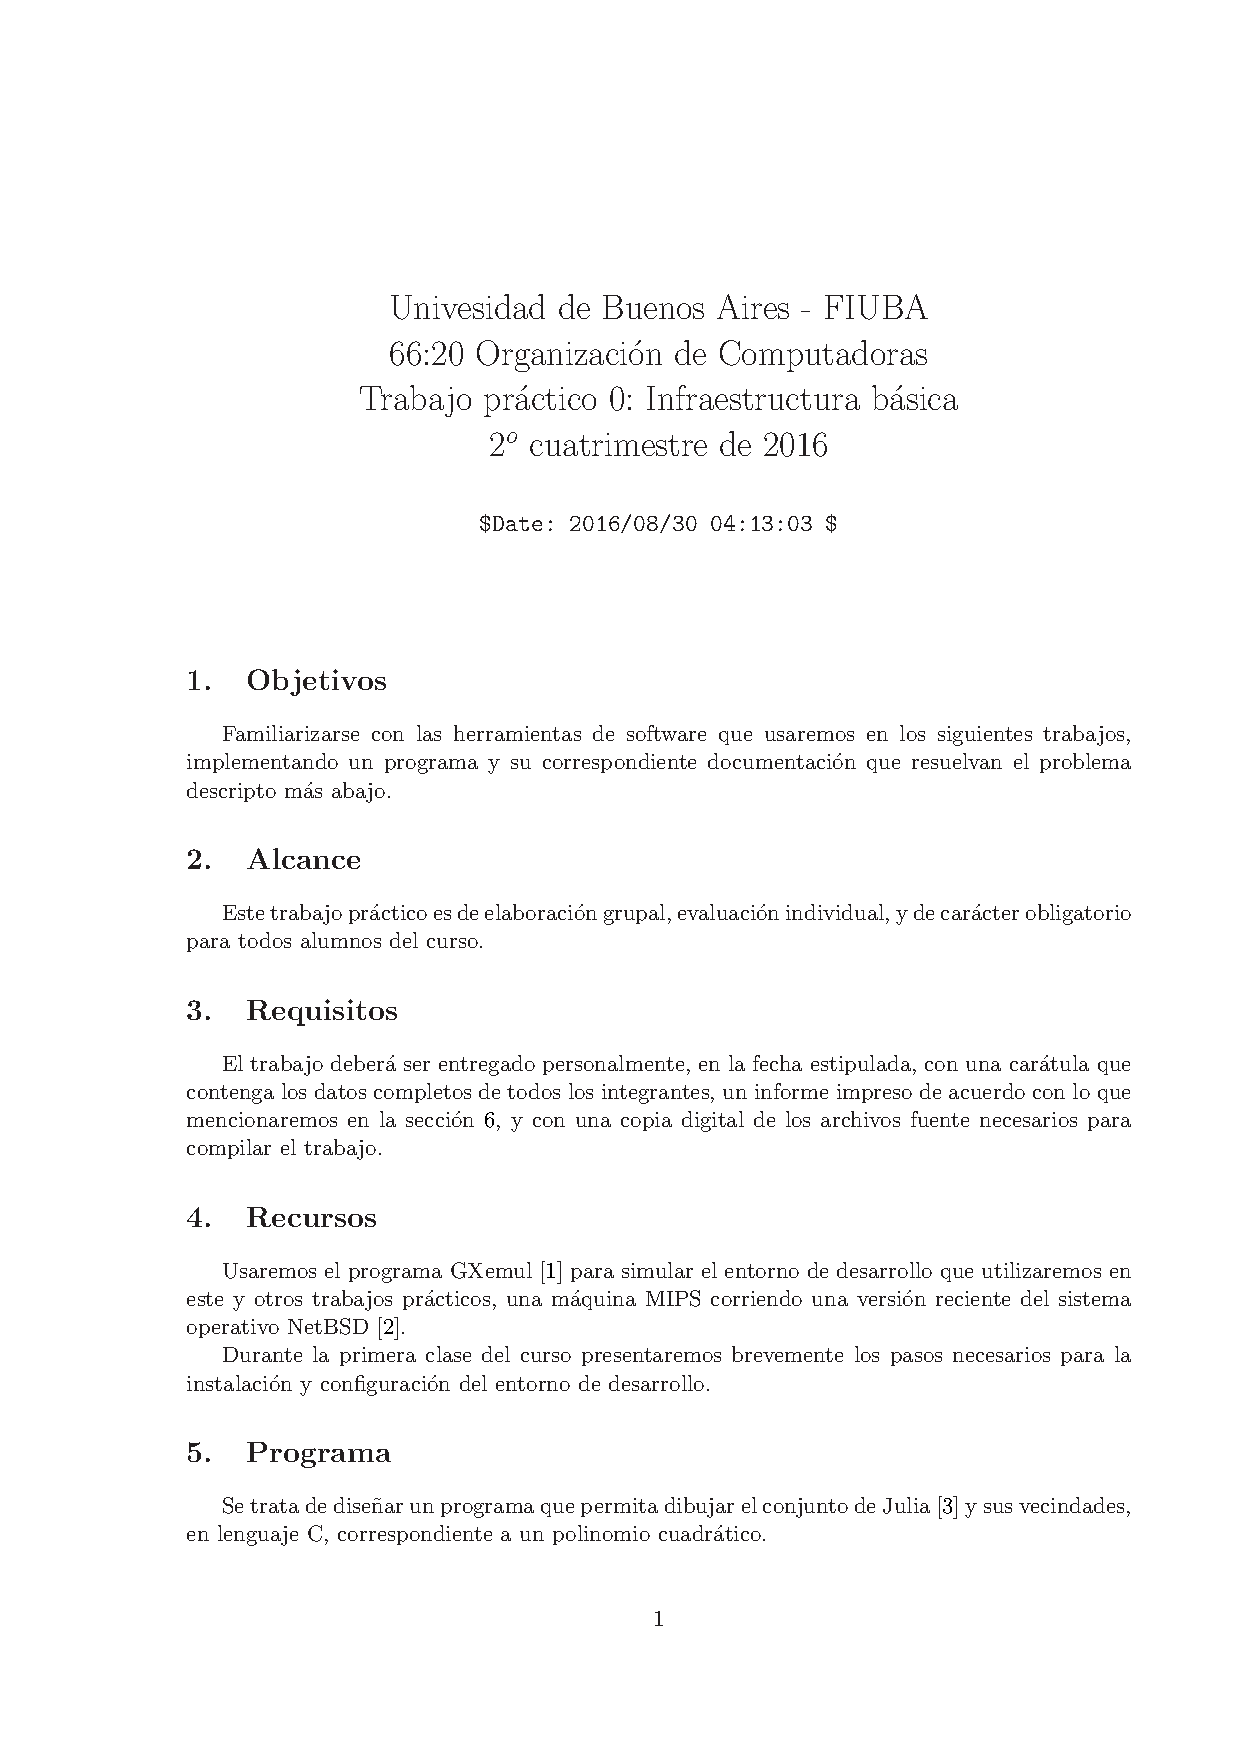
\includepdf[pages={-}]{enunciado.pdf}

\begin{thebibliography}{99}
\bibitem{Gxemul} \emph{GXemul}\\
\url{http://gavare.se/gxemul/}

\bibitem{NetBSD} \emph{The NetBSD project}\\
\url{http://www.netbsd.org/}

\bibitem{Juli} \emph{Conjunto de Julia}\\
\url{https://es.wikipedia.org/wiki/Conjunto_de_Julia}

\bibitem{PGM} \emph{PGM format specification}\\
\url{http://netpbm.sourceforge.net/doc/pgm.html}

\end{thebibliography}
\end{document}
